\chapter{Introduction}\label{chapter:introduction}

Semiconductor lasers present a very cmpact compact, efficient and mass-producable solid state laser. They have many applications in everyday life and science, such as optical communication, data storage, printing, sensing, medical treatment, and pumping solid-state lasers.

A VECSEL (Vertical-External-Cavity Surface-Emitting Laser) is a type of semiconductor laser that emits light perpendicular to the surface of a semiconductor wafer1. Unlike a VCSEL (Vertical-Cavity Surface-Emitting Laser), which has a closed cavity within the wafer, a VECSEL has an external cavity that is formed by one or more optical elements outside the wafer23. This allows for more flexibility in designing the laser parameters, such as wavelength, output power, beam quality and pulse duration23.

Semiconductor lasers are a type of laser that use semiconductor materials as the gain medium. The gain medium is the part of the laser that amplifies the light by stimulated emission, which is the process of emitting photons with the same energy and phase as the incoming photons. Semiconductor lasers use direct band gap semiconductor materials, which have a small energy difference between the conduction band and the valence band. The conduction band is where electrons can move freely, and the valence band is where electrons are bound to atoms. When an electron jumps from the conduction band to the valence band, it releases a photon with an energy equal to the band gap. This photon can then stimulate another electron to jump and emit another photon, creating a chain reaction of amplification. Semiconductor lasers are very compact and efficient, and can be mass-produced and integrated with other electronic devices. They have many applications in everyday life and science, such as optical communication, data storage, printing, sensing, medical treatment, and pumping solid-state lasers.

Semiconductor lasers were first developed in the early 1960s as homogeneous junction lasers, which were pn junction diodes made on a single material1. The first semiconductor laser was demonstrated by Robert N. Hall and coworkers at the General Electric Research and Development Center in Schenectady, New York, in 19622. Around the same time, two other groups also demonstrated semiconductor lasers independently3. However, these early lasers could only operate at very low temperatures and with high currents, limiting their practical applications.

Since then, semiconductor lasers have undergone significant improvements in performance, efficiency, reliability, and diversity. Some of the key developments include heterojunction lasers, which use different materials for the active region and the cladding layers; quantum well lasers, which confine the electrons and holes in thin layers to enhance the optical gain; distributed feedback lasers, which use a periodic structure to provide wavelength-selective feedback; vertical cavity surface emitting lasers (VCSELs), which emit light perpendicular to the surface of the chip; and quantum cascade lasers, which use intersubband transitions in multiple quantum wells to generate mid-infrared or terahertz radiation.

A VECSEL is a type of semiconductor laser that is based on a VCSEL (Vertical Cavity Surface Emitting Laser), but with an external cavity. A VCSEL is a laser diode that emits light perpendicular to the surface of a semiconductor wafer, unlike conventional edge-emitting lasers that emit light from the edges of the wafer12. A VCSEL has a closed cavity within the wafer, which consists of two highly reflective mirrors (called distributed Bragg reflectors) that sandwich a thin layer of active material (called quantum wells) where the light is generated by stimulated emission312.


\section{Gain saturation}

Gain saturation describes a phenomenon that occurs when the active region of a laser is unable to maintain its gain as the pump power increases for high values. 

To study this behaviour, one measures the nonlinear behaviour of the reflectivity for an increasing amount of probe fluence, as can be seen in \cref{fig:gainSat}. To quantify this behaviour and gain some macroscopic parameters, a model based on the saturation of the absorber in a SESAM can be fitted to the data. 

\begin{equation}
    \centering
    R(F)=R_{ns} \frac{F_{sat}}{F} \ln\left\{1 + \frac{R_{ss}}{R_{ns}} \left[\exp{ \left(\frac{F}{F_{sat}}\right) } - 1\right]\right\} \exp{\left(-\frac{F}{F_2}\right)}
    \label{eq:model}
\end{equation}

The parameters from \cref{eq:model} are the saturation fluence $F_{sat}$, the small signal reflectivity $R_{ss}$, the nonsaturable reflectivity $R_{ns}$ and the roll-over parameter $F_{2}$.

The saturation fluence $F_{sat}$ is the fluence at which the reflectivity reduces to $1/e$ of its maximum. It also represents the point at which the population inversion inside the active region becomes saturated, therefore it is closely tied to the material properties of the active region.

The small signal reflectivity $R_{ss}$ refers to the reflectivity at low probe fluence, where the gain is not significantly saturated. In this regime nonlinear effects are minimal and the reflectivity can be consider the be in the linear regime and the small signal approximation can be applied and the small signal gain can be calculated as $g_{ss}=R_{ss}-100\%$.

The nonsaturable reflectivity $R_{ns}$ arises from absorption and scattering at impurities and interfaces inside the VECSEL structure. This limits the maximum performance of the VECSEL, thus reducing defect during the growing process is important. Since this effect is associated with imperfection and reflection inside the structure it remains relatively constant for different probe fluences. 

The roll-over parameter $F_2$ describes further absorption from two photon absorption or higher order effects resulting in a strong decrease in the reflectivity at high fluences.

\Cref{fig:gainSat} shows the key parameters and the fitted model with and without accounting for the roll-over for a measurement of a VECSEL with an integrated pump DBR.


\begin{figure}[ht]
    \centering
    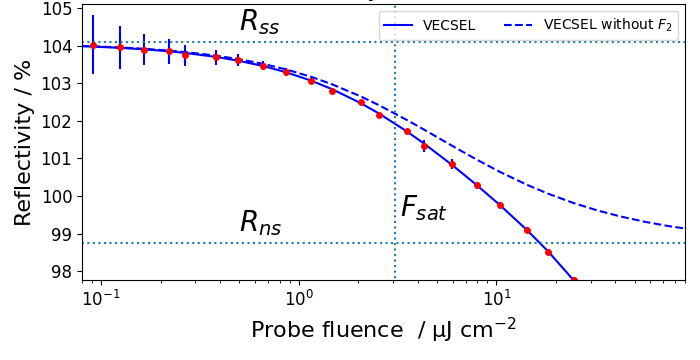
\includegraphics[width=12cm]{images/gainSat.png}
    \caption{Nonlinear reflectivity measurement for a diamond backed VECSEL with integrated pump DBR versus probe fluence. The data is shown with the fitted model utilizing \cref{eq:model} and the same model without the roll over parameter $F_2$. Additionally the different parameters $R_{ss}$, $R_{ns}$ and $F_{sat}$ are visualized.}
    \label{fig:gainSat}
\end{figure}

\section{VECSEL Chips}\label{sec:vecsel}

TODO: redo design images maybe with legend? different colors?

The basic structure of a VECSEl gain chip is shown in \cref{fig:vecDes}. The main feature of the structure are as follows: 

\begin{itemize}
    \item Heat spreader: The heat spreader role is in dissipating the heat generated during the operation of the VECSEL chip to a Peltier-controlled copper heat-sink.
    \item Pump \& laser  DBR: The purpose of the two bottom mirrors is to reflect the laser light and the pump light. There are two main advantages to this approach: firstly, because of higher absorption, there is a higher optical-to-optical efficiency due to the two passes through the active region, and secondly, there is less absorption in the mirror and in the heat sink, which results also in a higher efficiency and a higher maximum output power. The high reflectivity for two wavelengths is realized by using a distributed Bragg reflector (DBR)
    \item Active region: The purpose of the active region is the conversion of the pump light into the laser light. The gain medium in the active region is often composed of quantum wells or quantum dots.
    \item Anti-reflection coating: The antireflection section is optimized to reduce the otherwise large reflection from the air/GaAs interface
\end{itemize}

Below the three different structure of the Vecsel chips used in this work.

\begin{figure}[ht]
    \centering
    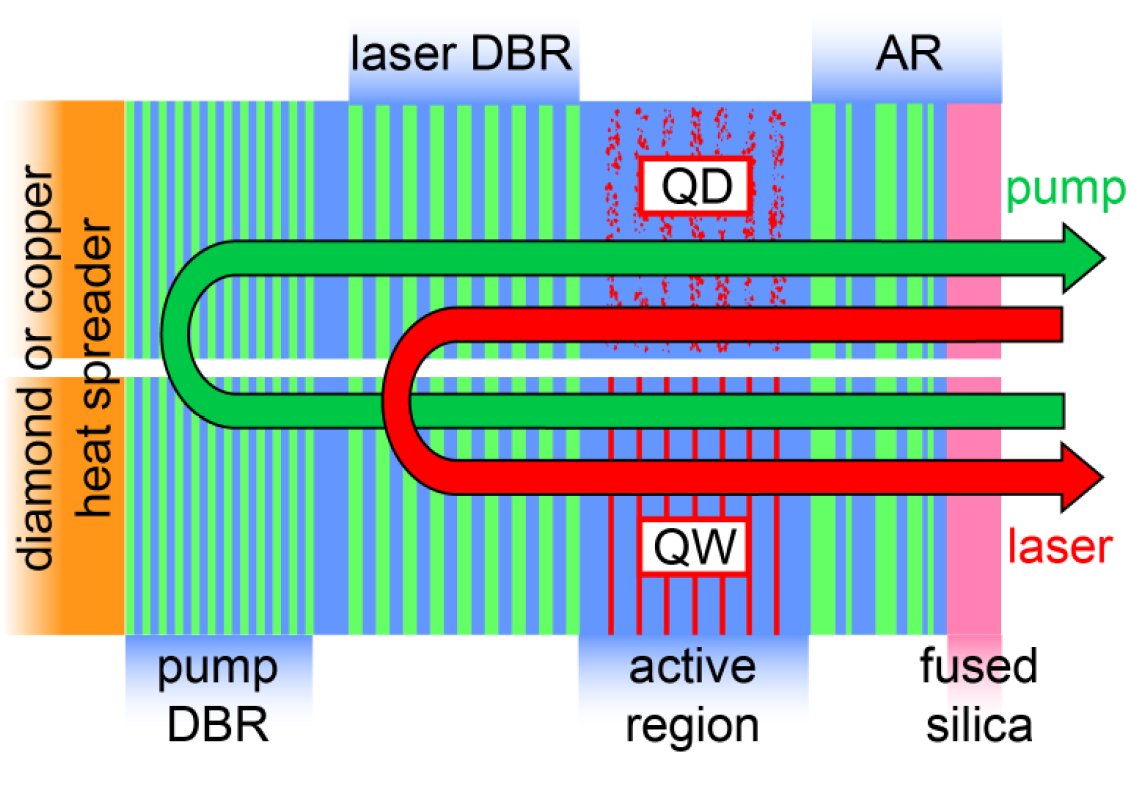
\includegraphics[width=.6\linewidth]{images/VECSEL_structure.png}
    \caption{TODO: caption}
    \label{fig:vecDes}
\end{figure}


%A distributed Bragg reflector (DBR) for the pump wavelength (808 nm) reflects the unabsorbed pump light, reducing heat deposition in the structure and increasing efficiency.
% The DBR for the laser wavelength acts as a flat cavity mirror.


\subsection*{No pump DBR chip, SV166}

\begin{wrapfigure}{r}{.4\textwidth}
    \vspace{-\baselineskip}
    \centering
    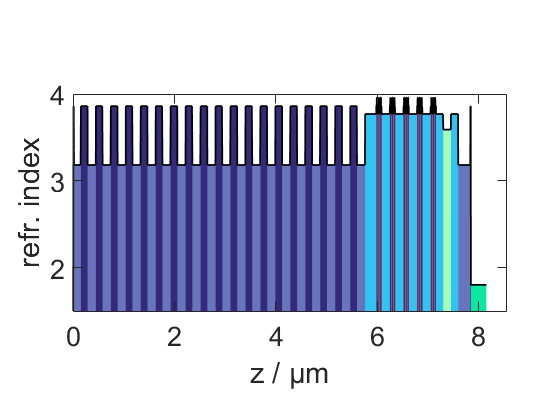
\includegraphics[width=.98\textwidth]{images/1SV166.lay.png}
    \caption{TODO: caption}
    \label{fig:sv166}
\end{wrapfigure}

This structure has an antiresonant design and cooled from the backside by a copper heat spreader. The DBR consists of 19-pairs of GaSb/AlAs\textsubscript{0.08}Sb\textsubscript{0.92} layers design around a wavelength of \qty{2080}{nm}. The active region has $5\times3$ In\textsubscript{0.27}Ga\textsubscript{0.73}Sb quantum wells (QW) placed at the maximum of the standing-wave cavity. Additional barriers layer made of AlAs\textsubscript{0.08}Sb\textsubscript{0.92} are placed around the gain QW to increase the photoluminesence. The last layer is a PECVD coating made of Si\textsubscript{3}N\textsubscript{4}, which serves an an antireflection coating.


\subsection*{Pump DBR chip, SV167}

\begin{wrapfigure}{r}{.4\textwidth}
    \vspace{-\baselineskip}
    \centering
    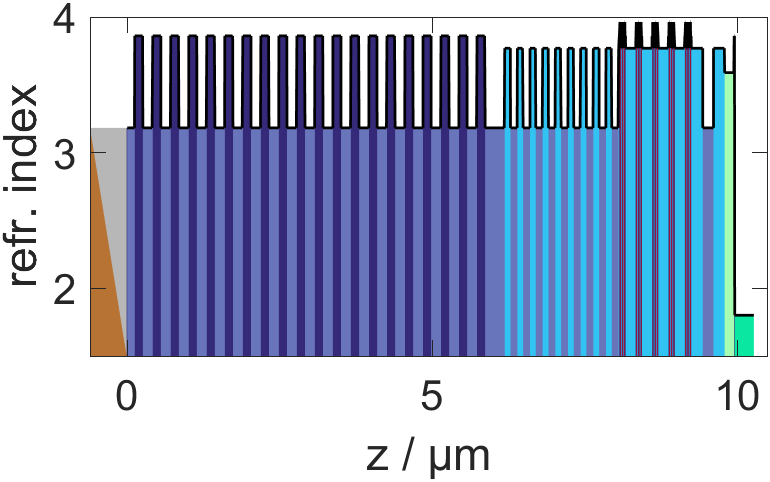
\includegraphics[width=.98\textwidth]{images/1SV167B.lay.png}
    \caption{TODO: caption}
    \label{fig:sv167}
\end{wrapfigure}

This is a similar strucutre as above but this time including an extra DBR for the pump wavelength of \qty{1470}{\nm}. The pump DBR is made of 10 layers of Al\textsubscript{0.2}As\textsubscript{0.8}Sb/Al\textsubscript{0.15}Ga\textsubscript{0.85}AsSb. For the thickness of the layers the \qty{45}{\degree} incident of the pump beam had to be accounted for. This strucutre was measured twice but for different heat spreaders, one made of copper and the other of diamond, to observe and compare the influence of better thermal conductovity of the heatsinks.


\subsection*{Hybrid chip, SV165}

\begin{wrapfigure}{r}{.4\textwidth}
    \vspace{-\baselineskip}
    \centering
    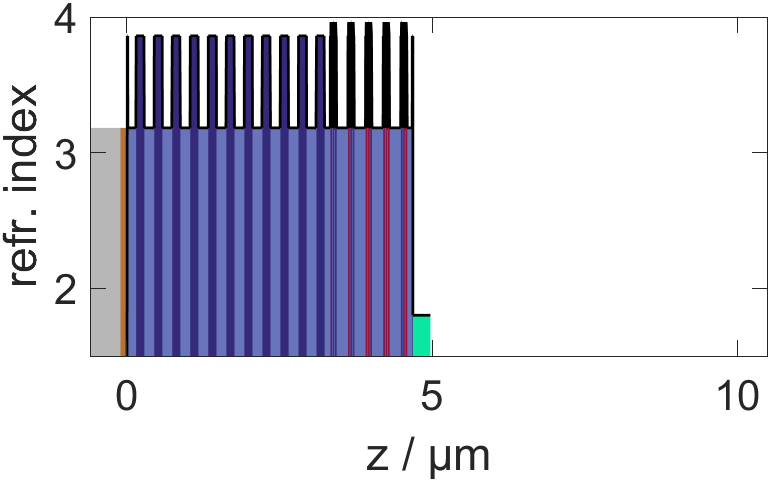
\includegraphics[width=.98\textwidth]{images/1SV165.lay.png}
    \caption{TODO: caption}
    \label{fig:sv165}
\end{wrapfigure}

This sturcutre incorbareted a hybrid metal-semiconductor Bragg reflector. It consisted of a  \qty{100}{\nm} copper layer with 10.5 AlAs\textsubscript{0.08}Sb\textsubscript{0.92}/GaSb layers. This allows for a thinner gain chip design of just under \qty{5}{\um} compared to the other strucutres \qty{7.5}{\um} resp. \qty{10}{\um} for the pump DBR design. This lowered the thermal resistance of the device by \qty{24}{\percent}. This structure also has a different active region made of $5\times3$ In\textsubscript{0.27}Ga\textsubscript{0.73}Sb/GaSb QW.
